\chapter{\textbf{ANÁLISE E RESULTADOS}}
\section{\textbf{Introdução à Análise de Resultados}}

Este capítulo apresenta a análise e discussão dos resultados obtidos no desenvolvimento do sistema de detecção de objetos e espaços no campus Pampulha da UFMG, com foco em sua aplicação como ferramenta assistiva para pessoas com deficiência visual. A avaliação tem como principal objetivo verificar a eficácia do modelo yolo11m.pt treinado com um \textit{dataset} personalizado, considerando tanto aspectos quantitativos quanto qualitativos do seu desempenho.

A análise está estruturada com base em artefatos gerados ao longo das fases de treinamento e validação do modelo, dentre os quais se destacam os gráficos de evolução das métricas durante as épocas, matrizes de confusão, curvas de \textit{precision}-\textit{recall}, medidas consolidadas de desempenho e exemplos visuais de detecção. Estes elementos possibilitam uma compreensão abrangente da capacidade do modelo em reconhecer corretamente as classes de interesse, banco, faixa de pedestre e placa de ônibus, sob diferentes condições ambientais.

Inicialmente, o capítulo aborda a caracterização do \textit{dataset} utilizado, detalhando sua composição e distribuição das classes. Em seguida, são analisadas as curvas de aprendizado do modelo, com foco na convergência das funções de perda e evolução das métricas. Na sequência, são apresentados os resultados quantitativos consolidados, seguidos por uma investigação mais minuciosa de erros e acertos por classe. Também são discutidas as relações entre o limiar de confiança e o comportamento das métricas de desempenho, com o auxílio de curvas \textit{Precision}-\textit{Recall} (PR) e \textit{F1-Score} (F1).

Complementarmente à análise numérica, são incluídas observações qualitativas baseadas em detecções reais em vídeos e imagens, buscando evidenciar situações práticas de acerto, erro e limitação do sistema. Por fim, é realizada uma discussão integrada dos resultados, com reflexões sobre o potencial do modelo como componente central de uma solução assistiva.

\section{\textbf{Caracterização do \textit{Dataset} e Configuração Detalhada do Treinamento}}

A qualidade e a representatividade do conjunto de dados são fatores determinantes para o desempenho de modelos baseados em aprendizado profundo, especialmente em aplicações de visão computacional. O \textit{dataset} utilizado neste trabalho foi construído com imagens capturadas no campus Pampulha da UFMG, abrangendo diferentes condições de luminosidade, horários do dia e contextos de ocupação do espaço. O objetivo foi garantir diversidade suficiente para permitir a generalização do modelo frente às variações ambientais do local de aplicação.

Foram definidas três classes de interesse, selecionadas com base em sua relevância para a orientação e segurança de pessoas com deficiência visual no contexto universitário: banco, faixa de pedestre e placa de ponto de ônibus. A distribuição dessas classes está ilustrada na Figura \ref{fg-labels}, com destaque para a predominância da classe banco, seguida por faixa de pedestre e, por fim, placa de ônibus. Embora o número de instâncias não seja equilibrado entre as classes, todas foram representadas em quantidade suficiente para permitir o aprendizado, considerando as boas práticas para \textit{datasets} personalizados de detecção de objetos.

% --- Figura
\begin{figure}[htbp]
  \centering
  \caption{Análise da distribuição das anotações e distribuição espacial das caixas delimitadoras no \textit{dataset}.}
  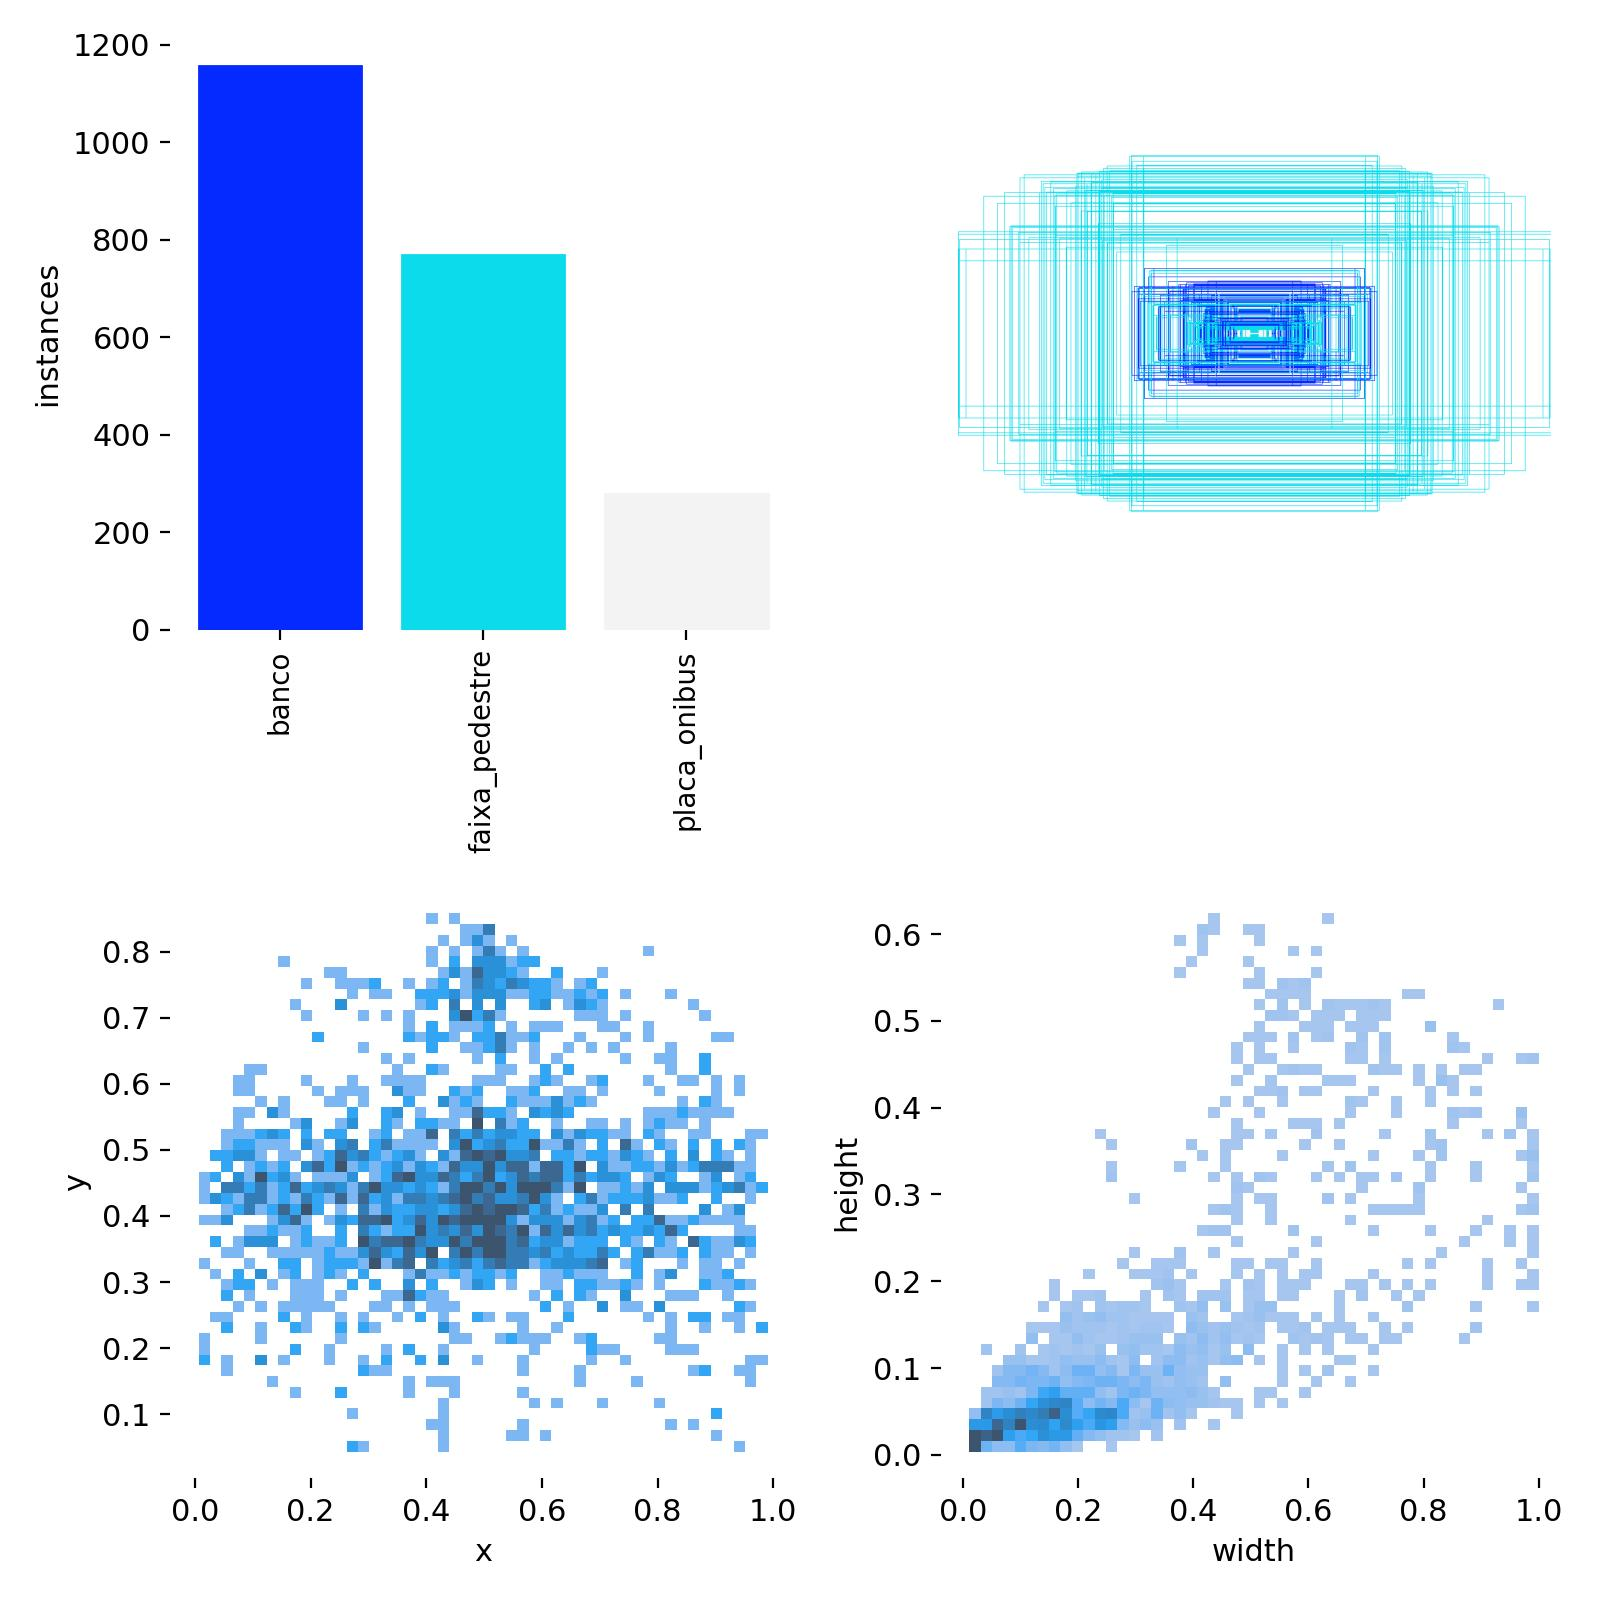
\includegraphics[width=0.8\textwidth]{Figuras/labels.jpg}
  \\
  Fonte: Autoral.
  \label{fg-labels}
\end{figure}
% --- Figura

A fim de aumentar a variabilidade das amostras e reduzir o risco de \textit{overfitting}, foi aplicada uma estratégia de \textit{data augmentation}, incluindo técnicas como espelhamento horizontal, ajustes de brilho e saturação, inserção de ruído e pequenas transformações geométricas. Com isso, o número total de imagens disponíveis para o treinamento foi expandido de aproximadamente 600 para 1444. Adicionalmente, as anotações foram realizadas de forma detalhada com auxílio da plataforma Roboflow, que também foi responsável pela divisão do \textit{dataset} em 88\% para o conjunto de treinamento e 12\% para validação.

A distribuição espacial das anotações nos \textit{frames} indica que os objetos foram capturados em diferentes posições e tamanhos dentro da imagem, o que é desejável para a aprendizagem de um detector robusto. A variedade nas dimensões e localizações das caixas delimitadoras reforça a heterogeneidade do conjunto, permitindo ao modelo aprender a identificar os objetos independentemente de sua escala, orientação ou posição no campo visual.

O processo de treinamento foi conduzido com base na arquitetura YOLOv11, utilizando pesos pré-treinados (modelo yolo11m.pt) como ponto de partida. A execução ocorreu em ambiente Google Colab, com o uso de uma GPU NVIDIA Tesla T4. As imagens foram redimensionadas para 640x640 pixels, e o treinamento estendeu-se por 80 épocas. A escolha automática do tamanho de batch (definido como -1) resultou em lotes de 14 imagens, considerando as limitações da GPU disponível.

A configuração dos hiperparâmetros foi gerenciada pela biblioteca Ultralytics, com a seleção automática do otimizador AdamW e de uma taxa de aprendizado ajustável. Essa automatização visou otimizar o processo para os recursos computacionais disponíveis e acelerar a convergência do modelo. A Figura \ref{fg-labels} também apresenta a distribuição dos centros e tamanhos das caixas, reforçando a diversidade de exemplos que alimentaram o processo de aprendizado.

Em síntese, a construção criteriosa do \textit{dataset} e a configuração adequada do processo de treinamento formaram uma base sólida para os resultados apresentados nas seções subsequentes. A diversidade de cenários contemplados, aliada ao uso de técnicas de \textit{data augmentation}, contribuiu significativamente para a robustez do modelo treinado frente às condições reais de aplicação no ambiente universitário.

\section{\textbf{Análise do Processo de Convergência do Modelo durante o Treinamento}}

A análise das curvas de convergência durante o treinamento do modelo yolo11m.pt fornece informações essenciais sobre a eficácia do processo de aprendizado e sobre a estabilidade das métricas de desempenho ao longo das épocas. A Figura \ref{fg-results} compila os gráficos gerados pela biblioteca Ultralytics, apresentando a evolução das funções de perda e métricas de \textit{precision} e \textit{recall} tanto para o conjunto de treinamento quanto para o conjunto de validação.

% --- Figura
\begin{figure}[htbp]
  \centering
  \caption{Evolução das métricas de perda (box, cls, dfl) e \textit{Mean Average Precision} (mAP50, mAP50-95) nos conjuntos de treinamento (linha superior) e validação (linha inferior) ao longo das 80 épocas de treinamento do modelo}
  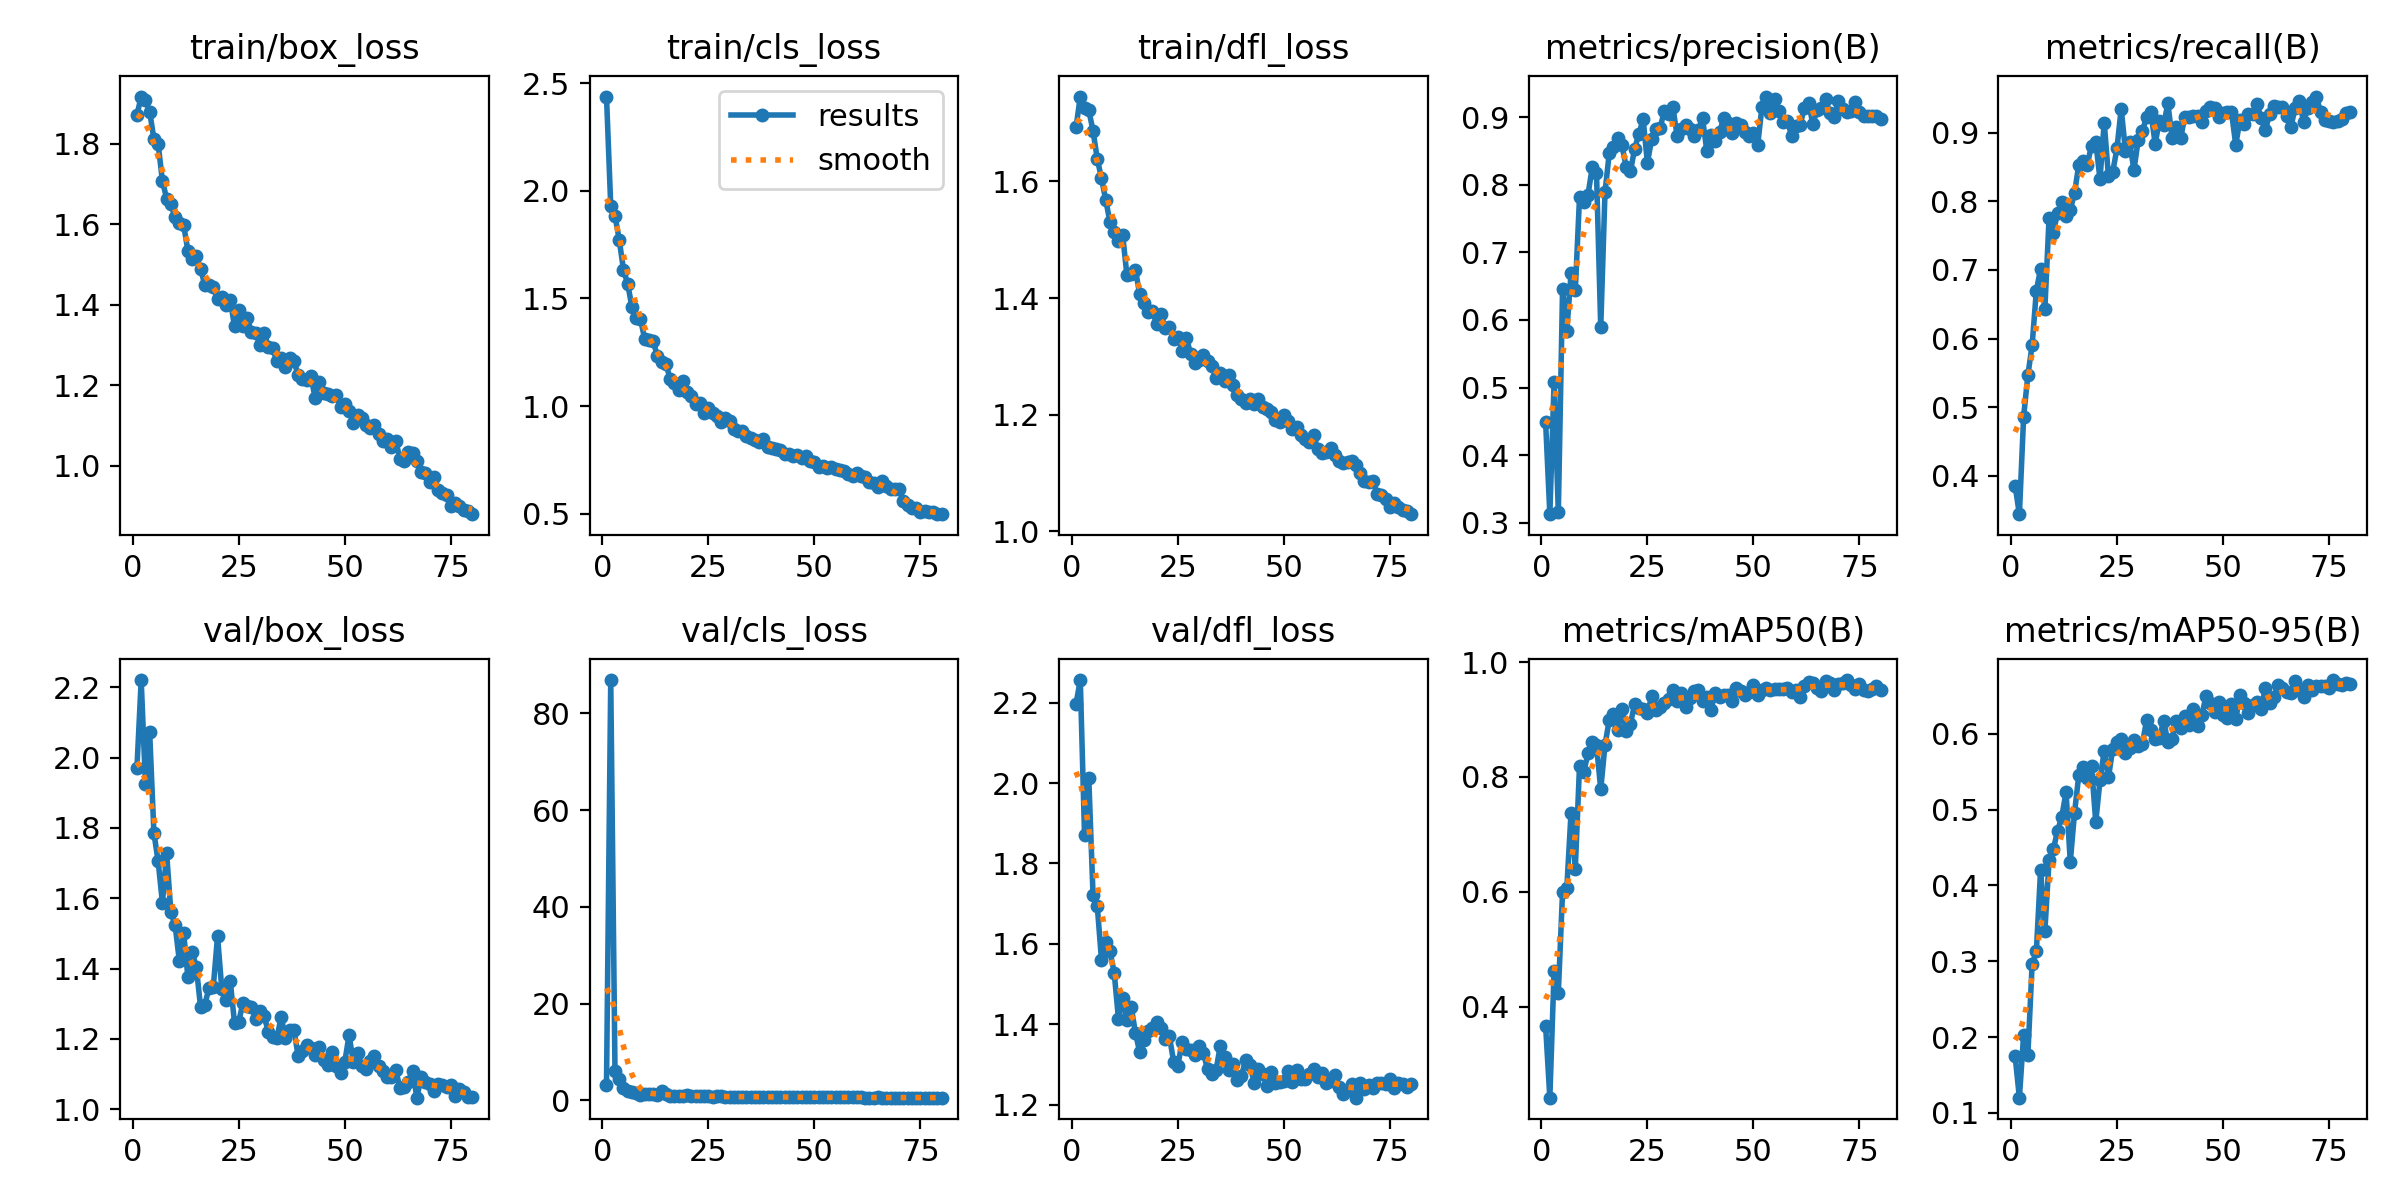
\includegraphics[width=1\textwidth]{Figuras/results.png}
  \\
  Fonte: Autoral.
  \label{fg-results}
\end{figure}
% --- Figura

Observa-se nas curvas de perda (\textit{box\_loss}, \textit{cls\_loss} e \textit{dfl\_loss}) um comportamento típico de convergência eficiente: redução acentuada nas primeiras 30 épocas, seguida de estabilização progressiva até aproximadamente a 75ª época. Este padrão é evidência de que o modelo ajustou adequadamente seus parâmetros iniciais, entrando posteriormente em uma fase de refinamento gradual. A ausência de oscilações abruptas ou aumentos nas curvas de perda valida a consistência do processo e a adequação da taxa de aprendizado empregada.

As curvas referentes ao conjunto de validação acompanham de forma coesa as do treinamento, sem divergências significativas entre elas. Essa proximidade indica que o modelo não sofreu \textit{overfitting} durante as 80 épocas, mantendo sua capacidade de generalização para dados não vistos. A semelhança entre os comportamentos dos dois conjuntos também sugere que as técnicas de regularização adotadas, aliadas à diversidade do \textit{dataset}, foram eficazes para a estabilização do processo.

Em relação às métricas de desempenho, destacam-se os valores progressivamente crescentes de mAP@0.5 e mAP@0.5:0.95. A métrica mAP@0.5 ultrapassou o valor de 0.90 antes da 50ª época, estabilizando-se em torno de 0.94 nas últimas iterações. Já a métrica mAP@0.5:0.95, mais rigorosa, apresentou crescimento contínuo, atingindo valores superiores a 0.70. Ambos os resultados são indicadores de desempenho elevado, considerando-se o contexto de aplicação e o volume de dados utilizados.

As métricas de \textit{precision} e \textit{recall} apresentaram curvas consistentes com o comportamento das perdas. Em particular, o \textit{recall} manteve-se elevado ao longo das últimas épocas, evidenciando a capacidade do modelo de detectar a maioria dos objetos presentes nas imagens. A \textit{precision}, por sua vez, apresentou estabilidade após a 40ª época, refletindo o equilíbrio alcançado entre acertos e falsos positivos.

Conclui-se, com base nas curvas de aprendizado e desempenho, que o modelo convergiu de forma eficaz dentro do intervalo estipulado de 80 épocas. A ausência de comportamento instável, a aproximação entre os conjuntos de treinamento e validação e os altos valores de mAP consolidam a confiabilidade do processo de treinamento, justificando a seleção do modelo gerado como base para as avaliações quantitativas e qualitativas posteriores.

\section{\textbf{Avaliação Quantitativa de Desempenho do Modelo Final}}

Finalizado o treinamento, o modelo yolo11m.pt foi avaliado por meio da aplicação do conjunto de pesos otimizados (arquivo best.pt) sobre o subconjunto de validação do \textit{dataset}, contendo 178 imagens e 306 instâncias. Essa validação foi conduzida com a ferramenta Ultralytics, utilizando o comando específico em modo val, responsável por calcular as métricas consolidadas de desempenho para cada classe. Os resultados estão organizados na Tabela \ref{tab:metricas-yolov11m}, que resume as métricas de \textit{precision}, \textit{recall}, mAP@0.5 e mAP@0.5:0.95 por classe e no total.

\begin{table}[htbp]
\centering
\caption{Métricas de desempenho do modelo \texttt{yolo11m.pt} (best.pt) no conjunto de validação}
\label{tab:metricas-yolov11m}
\resizebox{\textwidth}{!}{%
\begin{tabular}{lcccccc}
\toprule
\textbf{Classe} & \textbf{Imagens} & \textbf{Instâncias} & \textbf{\textit{Precision}} (P) & \textbf{\textit{Recall}} (R) & \textbf{mAP@0.5} & \textbf{mAP@0.5:0.95} \\
\midrule
Todas (média)   & 178               & 306                 & 0.927                 & 0.936               & 0.967            & 0.670               \\
Banco           & 67               & 152                  & 0.859                 & 0.941               & 0.942            & 0.681               \\
Faixa\_pedestre & 86               & 104                  & 0.921                 & 0.893               & 0.966            & 0.606               \\
Placa\_onibus   & 50               & 50                  & 1.000                 & 0.973               & 0.994            & 0.721               \\
\bottomrule
\end{tabular}%
}
\end{table}

A análise da média geral evidencia um desempenho expressivo do modelo. A \textit{precision} de 0.927 indica que, entre todas as detecções realizadas, aproximadamente 93\% foram corretas. O \textit{recall} de 0.936 demonstra que o modelo conseguiu identificar a grande maioria dos objetos presentes nas imagens. A métrica mAP@0.5, com valor de 0.967, confirma a alta acurácia da detecção com uma tolerância padrão de Intersecção sobre União (IoU) de 50\%. Já a mAP@0.5:0.95, com valor de 0.670, representa um resultado satisfatório mesmo sob critérios mais rígidos de correspondência entre predição e anotação.


No desempenho individual por classe, destaca-se a classe placa\_onibus, que atingiu \textit{precision} perfeita de 1.000, \textit{recall} de 0.973 e mAP@0.5:0.95 de 0.721 — o melhor entre todas as classes. Este resultado sugere que o modelo identificou com segurança e exatidão as placas de ponto de ônibus, possivelmente devido ao seu formato e cor característicos, que oferecem menor ambiguidade visual.

A classe faixa\_pedestre apresentou resultados igualmente positivos, com \textit{precision} de 0.921 e \textit{recall} de 0.893. O mAP@0.5 de 0.966 reflete o bom desempenho na detecção e delimitação espacial deste tipo de objeto, apesar de sua variabilidade de aparência e iluminação, especialmente sob diferentes condições de piso e sombra.

Já a classe banco, embora com métricas consideradas aceitáveis, apresentou o desempenho mais modesto. A \textit{precision} de 0.859 e o \textit{recall} de 0.941 indicam maior incidência de falsos positivos e negativos em relação às demais classes. O valor de mAP@0.5 de 0.942 confirma essa maior dificuldade, atribuível à diversidade de formas, tamanhos e materiais dos bancos encontrados no campus, além de sua frequente oclusão parcial por pessoas ou vegetação.

Ressalta-se que o conjunto de validação utilizado é limitado em tamanho, o que pode introduzir certa variabilidade estatística nos resultados. Ainda assim, os padrões observados são consistentes com as análises das curvas de treinamento (Figura \ref{fg-results}) e com as tendências verificadas na matriz de confusão (próxima seção). A velocidade de inferência, próxima de 23 ms por imagem na GPU Tesla T4, também reforça a viabilidade do modelo para aplicações em tempo real.

Em resumo, os resultados quantitativos obtidos confirmam que o modelo yolo11m.pt treinado apresenta desempenho compatível com aplicações práticas de suporte à navegação assistiva, oferecendo boa acurácia de detecção, baixo índice de erro e estabilidade frente a dados não vistos.

\section{\textbf{Análise Detalhada de Erros e Acertos com Base na Matriz de Confusão}}

A matriz de confusão é uma ferramenta essencial para a avaliação detalhada do desempenho de modelos de classificação, permitindo a identificação dos padrões de acertos e erros em cada classe individualmente. No contexto do modelo, essa análise revela não apenas a eficácia do algoritmo na classificação correta dos objetos, mas também os pontos de maior vulnerabilidade, especialmente no que diz respeito à distinção entre objetos de interesse e o fundo (\textit{background}).

A Figura \ref{fg-confusion_matrix} apresenta a matriz de confusão bruta, evidenciando a contagem absoluta das classificações feitas pelo modelo durante a validação. Os valores ao longo da diagonal principal indicam as classificações corretas, ou seja, os verdadeiros positivos (TP) para cada classe. Os valores fora da diagonal, por sua vez, representam erros de classificação, como falsos positivos (FP) e falsos negativos (FN). Observa-se que o modelo não apresentou confusões entre as classes-alvo, como por exemplo classificar um banco como faixa de pedestre. Isso demonstra uma clara capacidade discriminativa entre as classes definidas no \textit{dataset} personalizado.

% --- Figura
\begin{figure}[htbp]
  \centering
  \caption{Matriz de Confusão com contagens absolutas das predições no conjunto de validação do treinamento do modelo}
  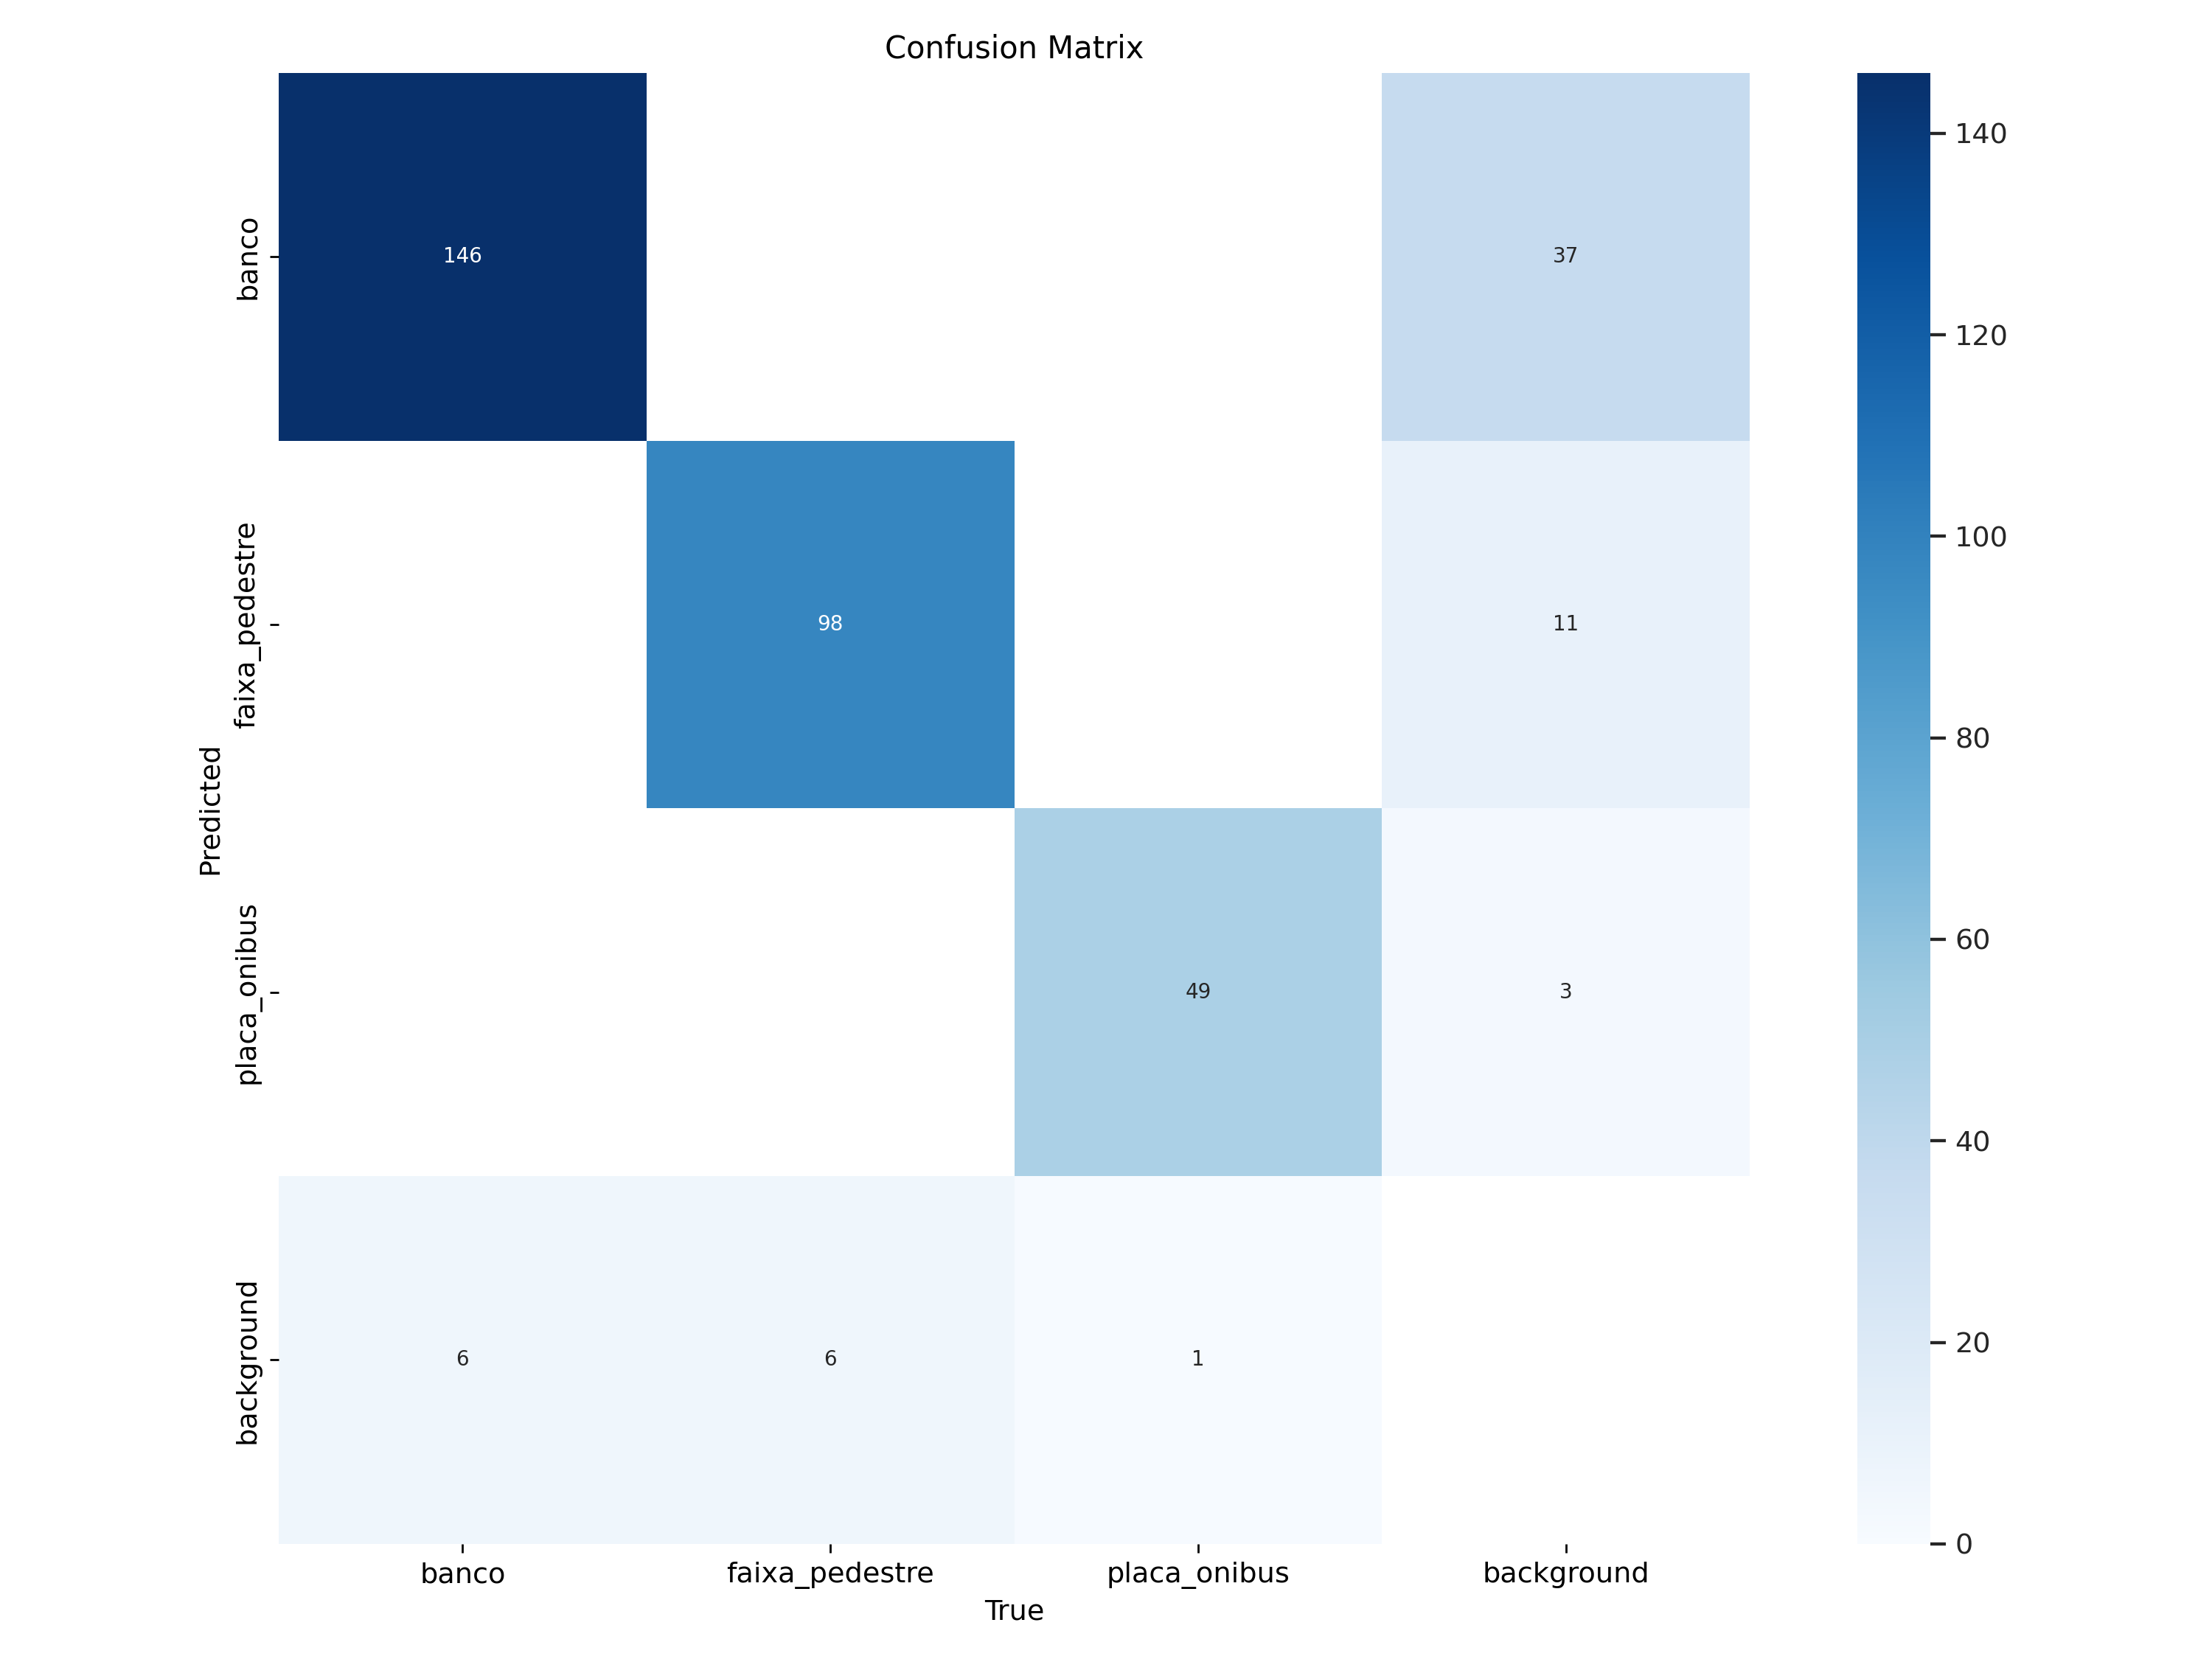
\includegraphics[width=1\textwidth]{Figuras/confusion_matrix.png}
  \\
  Fonte: Autoral.
  \label{fg-confusion_matrix}
\end{figure}
% --- Figura

No entanto, as maiores ocorrências de erros concentram-se na relação com o \textit{background}. Foram observados 37 falsos positivos para a classe banco, 11 para faixa\_pedestre e apenas 3 para placa\_onibus. Isso indica que o modelo, em algumas situações, interpretou elementos visuais do ambiente como objetos de interesse, quando na realidade tratava-se de elementos do cenário não anotados. Tais erros podem ser atribuídos a texturas ou estruturas visuais semelhantes aos objetos de interesse, como sombras, muros ou áreas pavimentadas com padrões similares.

A análise da matriz de confusão normalizada (Figura \ref{fg-confusion_matrix_normalized}) oferece uma visualização mais intuitiva do \textit{recall} por classe, ou seja, a proporção de objetos reais corretamente identificados pelo modelo. Os resultados indicam um desempenho elevado: banco com 96\%, faixa\_pedestre com 9\% e placa\_onibus com 98\%. Esses valores confirmam que o modelo possui uma elevada sensibilidade, sendo capaz de detectar a maioria dos objetos de cada categoria. Os erros restantes (FN) são geralmente atribuídos a condições adversas, como baixa iluminação, oclusões ou aparências incomuns dos objetos.

% --- Figura
\begin{figure}[htbp]
  \centering
  \caption{Matriz de Confusão Normalizada (valores da diagonal representam o \textit{Recall} por classe)}
  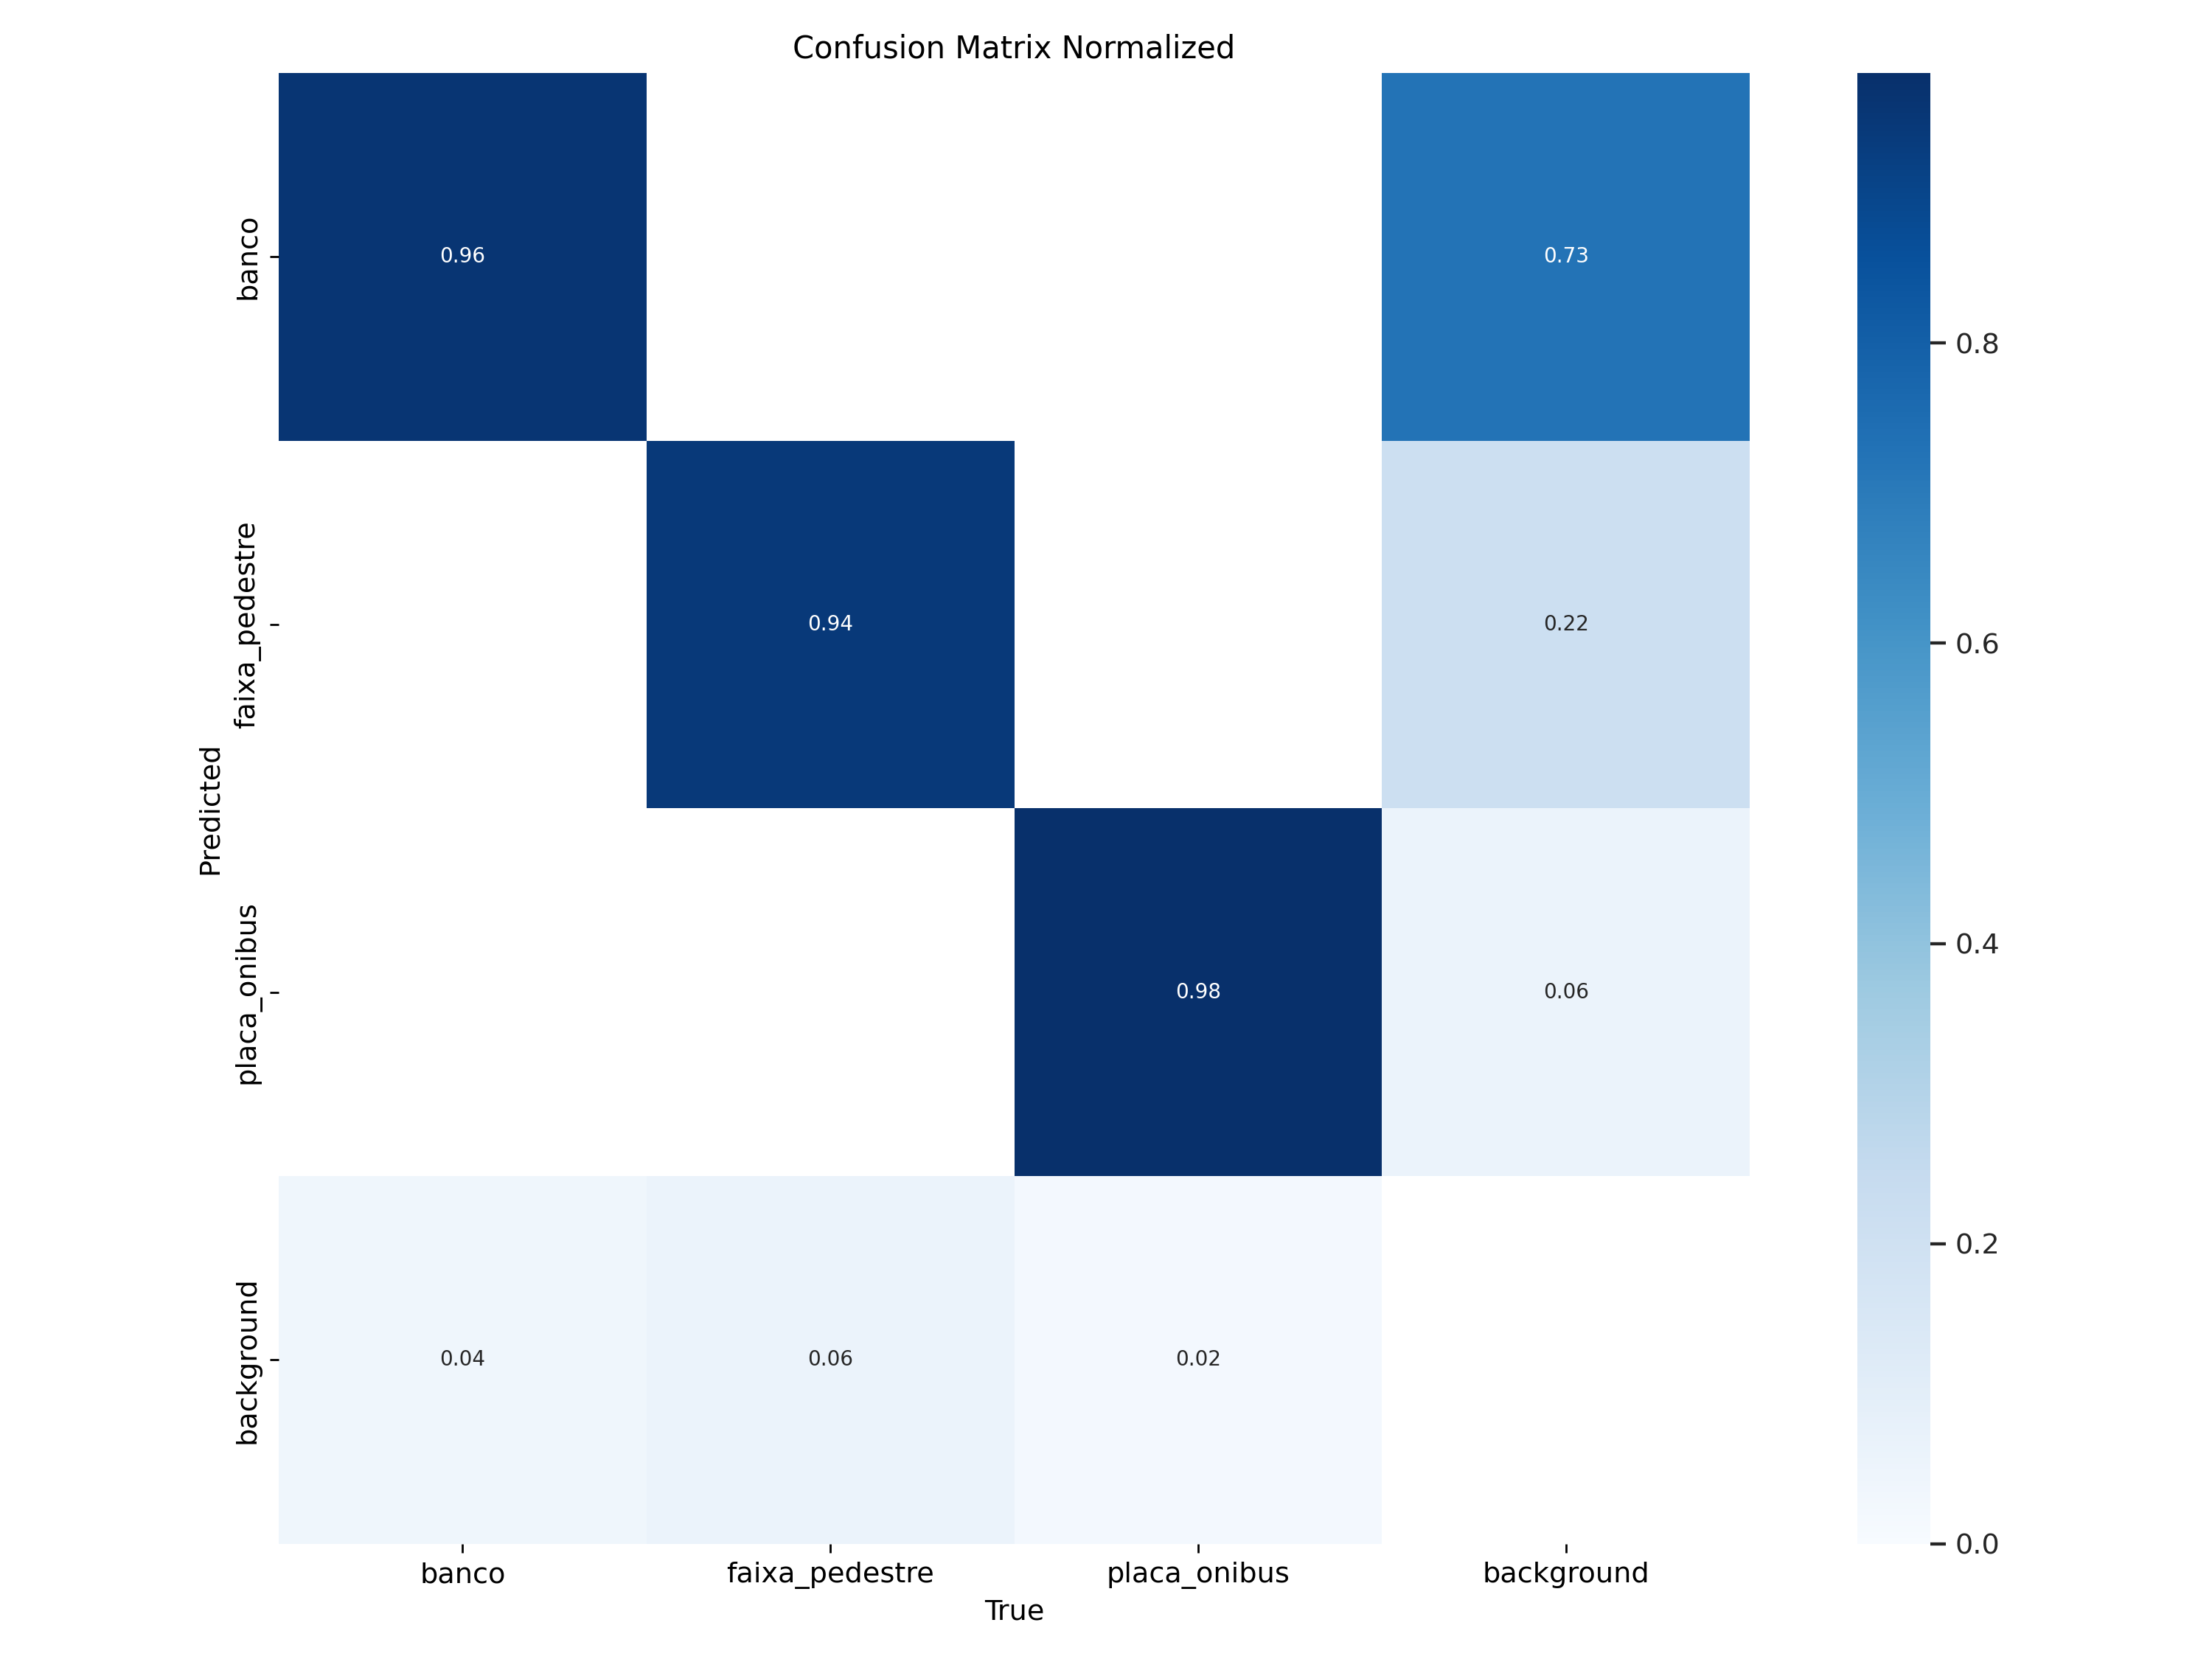
\includegraphics[width=1\textwidth]{Figuras/confusion_matrix_normalized.png}
  \\
  Fonte: Autoral.
  \label{fg-confusion_matrix_normalized}
\end{figure}
% --- Figura

A classe banco, apesar de apresentar um bom desempenho geral, foi a que mais acumulou falsos positivos. Isso sugere a necessidade de refinamento adicional, seja por meio da inclusão de exemplos negativos (\textit{background}s semelhantes a bancos) no \textit{dataset}, seja pela calibragem mais cuidadosa do limiar de confiança durante a inferência. Essa medida pode ajudar a minimizar alertas incorretos na aplicação final assistiva, sem comprometer o \textit{recall} da classe.

Em síntese, a análise das matrizes de confusão reforça que o modelo é confiável para aplicações práticas, demonstrando altos índices de acerto e baixa taxa de confusão entre classes. As limitações identificadas são pontuais e passíveis de aprimoramento, sem comprometer a viabilidade da ferramenta assistiva.


\section{\textbf{Relação entre Limiar de Confiança, \textit{Precision}, \textit{Recall} e \textit{F1-Score}}}

O desempenho de modelos de detecção de objetos é influenciado diretamente pelo limiar de confiança utilizado na inferência. Esse parâmetro define o grau mínimo de certeza que o modelo deve ter para considerar uma detecção como válida. Assim, ajustes nesse valor afetam diretamente o equilíbrio entre \textit{precision} (proporção de detecções corretas entre as detectadas) e \textit{recall} (proporção de detecções corretas entre as existentes). A análise das curvas PR e F1 permite entender essa dinâmica de maneira visual e quantitativa.

A Figura \ref{fg-pr_curve} apresenta as curvas PR para cada uma das classes, bem como para a média geral do modelo. Essas curvas ilustram o comportamento da \textit{precision} em função do aumento do \textit{recall}. Curvas que se mantêm próximas do canto superior direito do gráfico indicam um desempenho superior, com alta \textit{precision} mesmo quando o \textit{recall} é elevado. No presente modelo, observou-se que todas as classes apresentam curvas com esse comportamento desejável, com destaque para a classe placa\_onibus, que manteve \textit{precision} elevada em quase toda a faixa de \textit{recall}.

% --- Figura
\begin{figure}[htbp]
  \centering
  \caption{Curvas \textit{Precision}-\textit{Recall} para cada classe e para a média de todas as classes (mAP@0.5) no conjunto de validação do treinamento do modelo}
  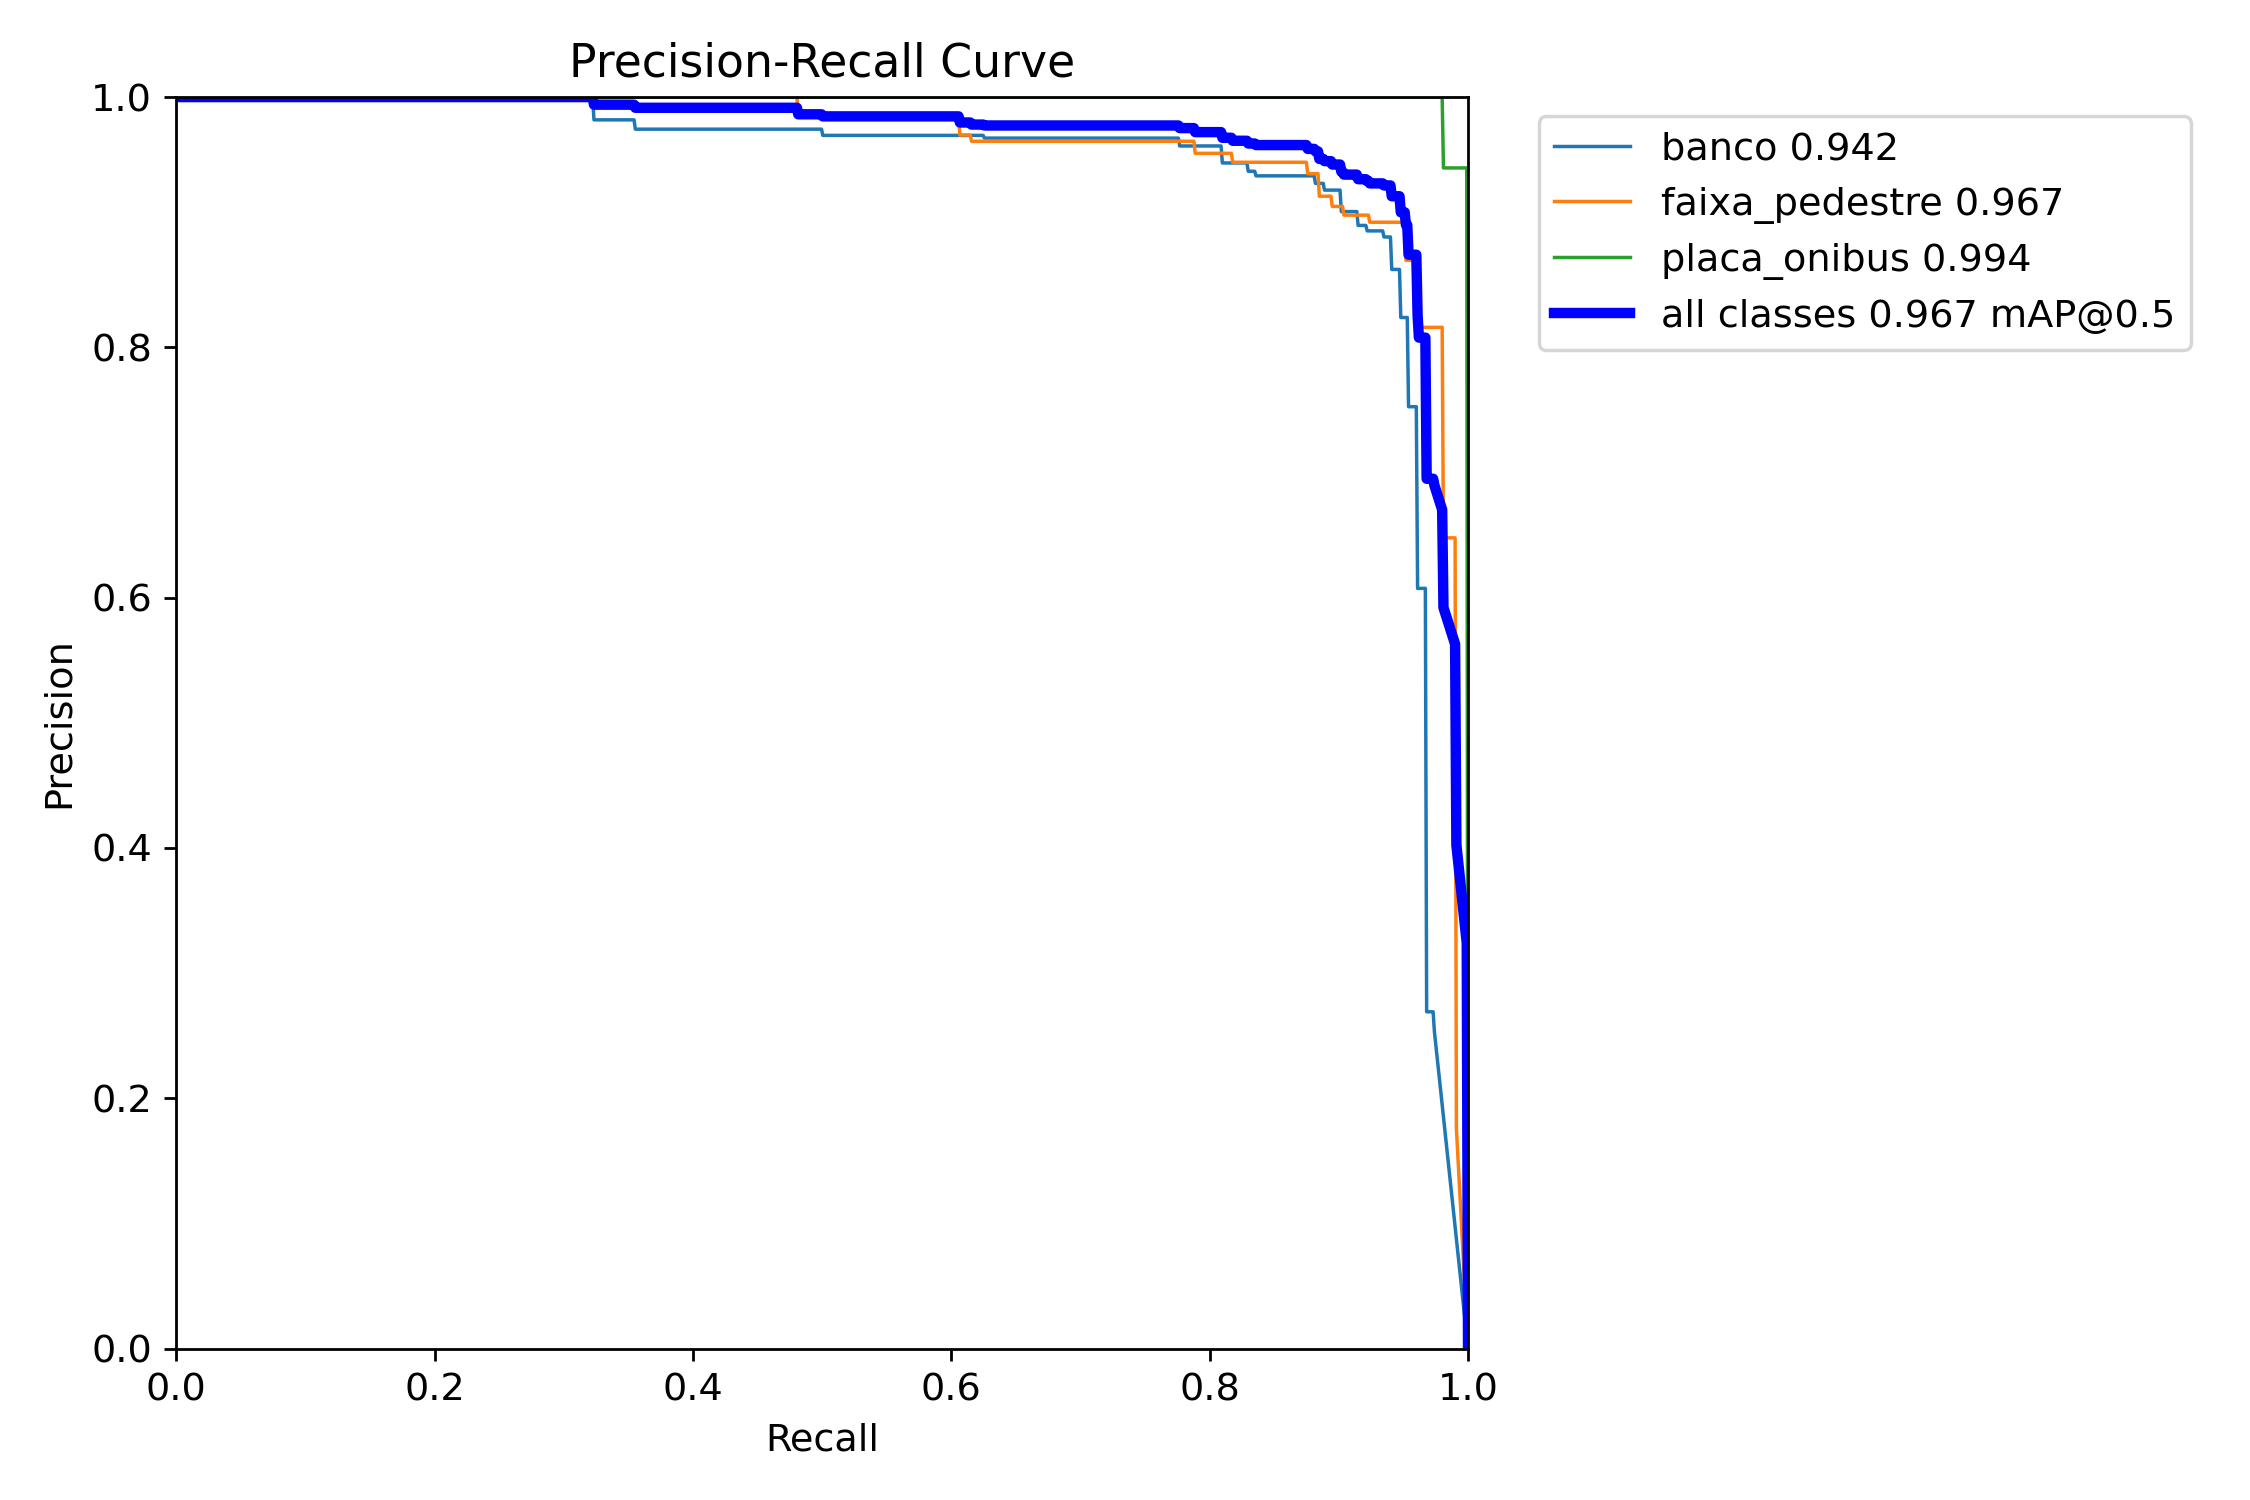
\includegraphics[width=1\textwidth]{Figuras/PR_curve.png}
  \\
  Fonte: Autoral.
  \label{fg-pr_curve}
\end{figure}
% --- Figura

Os valores de \textit{average precision} (AP) extraídos das curvas são bastante expressivos: 0.942 para banco, 0.967 para faixa\_pedestre e 0.994 para placa\_onibus. Esses resultados refletem a alta eficácia do modelo, especialmente considerando que foram obtidos com um \textit{dataset} personalizado e em ambiente não controlado. O AP médio de 0.967 indica que o modelo mantém um equilíbrio adequado entre \textit{precision} e \textit{recall} na maioria das situações.

A Figura \ref{fg-f1_curve} complementa a análise ao mostrar o comportamento do \textit{F1-Score} em função do limiar de confiança. O \textit{F1-Score} é uma métrica harmônica entre \textit{precision} e \textit{recall}, sendo especialmente útil para identificar o ponto ótimo de operação do modelo. Observa-se que o ponto de \textit{F1-Score} máximo para o modelo geral ocorre em torno de um limiar de 0.404, indicando que esse valor proporciona o melhor equilíbrio entre detectar objetos corretamente e evitar detecções incorretas.

% --- Figura
\begin{figure}[htbp]
  \centering
  \caption{Curvas do \textit{F1-Score} em função do Limiar de Confiança para cada classe e para a média de todas as classes no conjunto de validação do treinamento do modelo}
  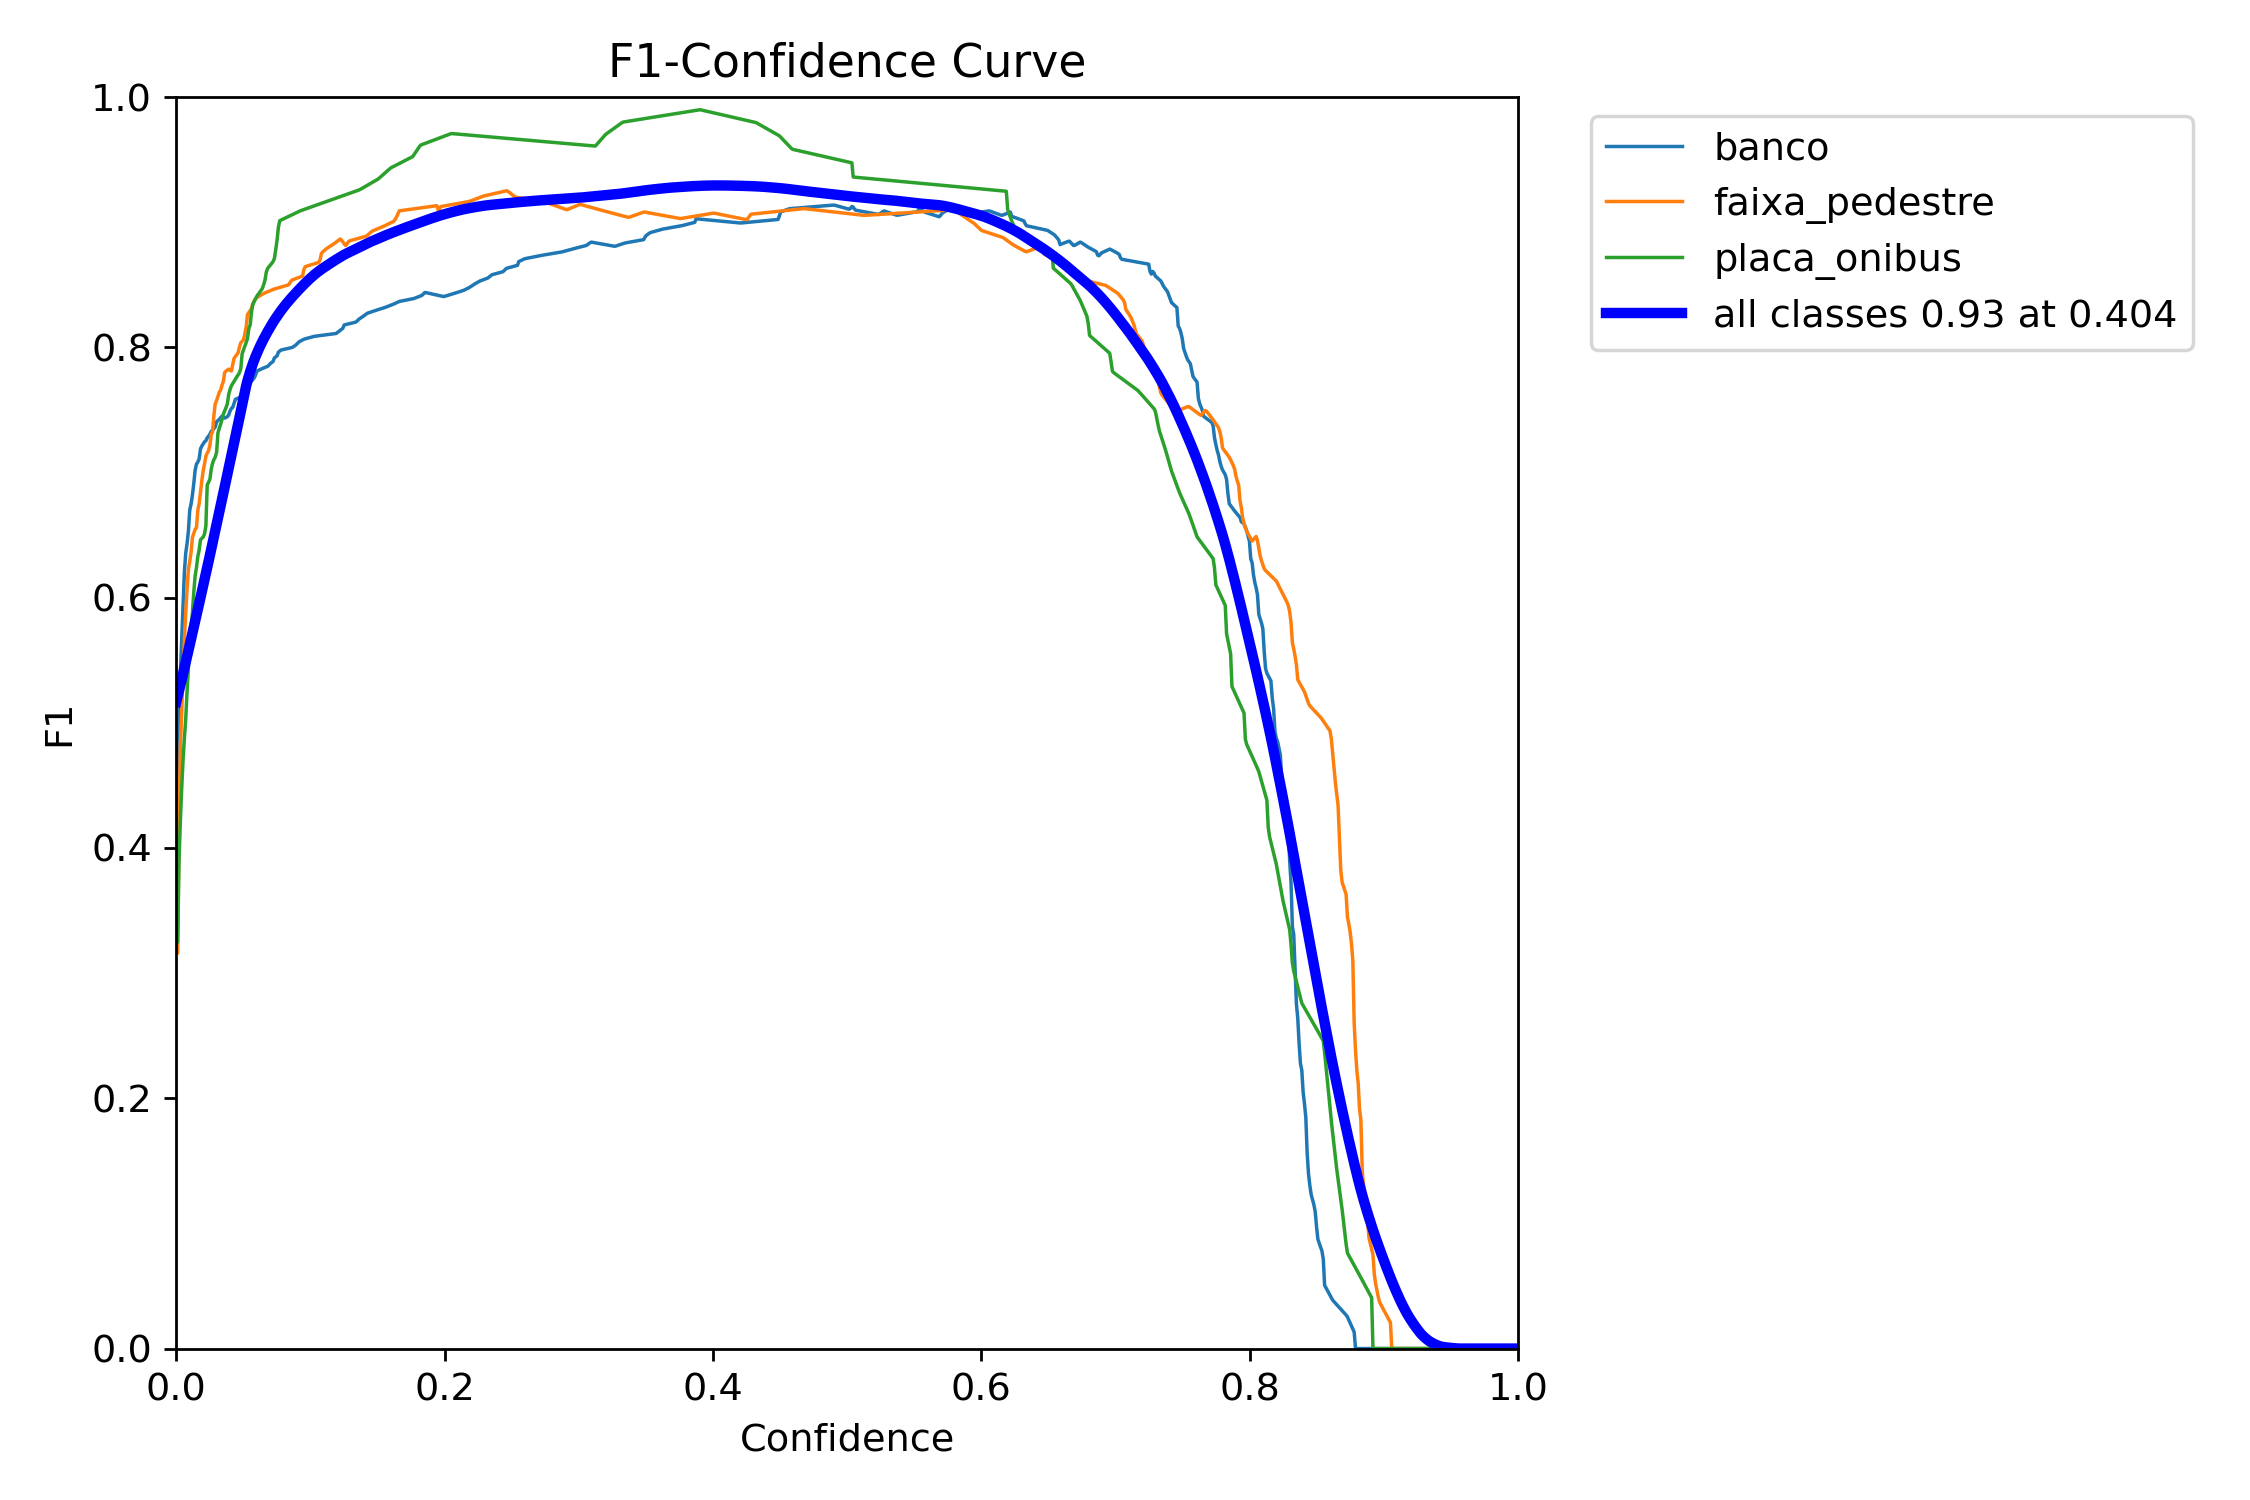
\includegraphics[width=1\textwidth]{Figuras/F1_curve.png}
  \\
  Fonte: Autoral.
  \label{fg-f1_curve}
\end{figure}
% --- Figura

Analisando individualmente as curvas de \textit{F1-Score} por classe, percebe-se que placa\_onibus mantém seu desempenho robusto mesmo em limiares mais altos, refletindo sua maior facilidade de detecção. Já as curvas de banco e faixa\_pedestre apresentam maiores variações, com picos de desempenho entre 0.35 e 0.55 de confiança, o que pode orientar o ajuste fino desses valores na aplicação prática.

Em termos de aplicação, especialmente em contextos assistivos, um maior \textit{recall} pode ser preferível, mesmo ao custo de alguns falsos positivos, desde que não comprometa a confiança do usuário no sistema. Assim, as curvas apresentadas servem não apenas como indicadores de desempenho, mas também como ferramentas de calibração para o uso prático do modelo.

\section{\textbf{Análise Qualitativa das Detecções em Cenários do Campus UFMG}}

Para além dos indicadores quantitativos, a análise qualitativa das detecções é fundamental para compreender a atuação prática do modelo em ambientes reais. Essa abordagem permite observar a qualidade visual das caixas delimitadoras, a confiabilidade das detecções em condições variadas e identificar situações específicas em que ocorrem erros, como falsos positivos ou falsos negativos, que podem não ser plenamente capturados pelas métricas agregadas.

A Figura \ref{fg-exemplo-deteccao-dia} apresenta um exemplo de detecção bem-sucedida, capturado durante o dia em local iluminado do campus Pampulha da UFMG. É possível observar múltiplas instâncias das classes de interesse sendo detectadas corretamente e com altos níveis de confiança (superiores a 0.80). As caixas delimitadoras são visualmente adequadas, envolvendo os objetos de forma precisa, com margens equilibradas e sem sobreposição excessiva com o fundo. Este resultado evidencia a capacidade do modelo em reconhecer simultaneamente diferentes objetos com confiabilidade, mesmo em ambientes dinâmicos, e reforça os elevados valores de \textit{precision} e mAP obtidos nas análises anteriores.

% --- Figura
\begin{figure}[htbp]
  \centering
  \caption{Exemplo de detecções corretas e bem localizadas para as classes banco e faixa\_pedestre em um cenário diurno no campus UFMG.}
  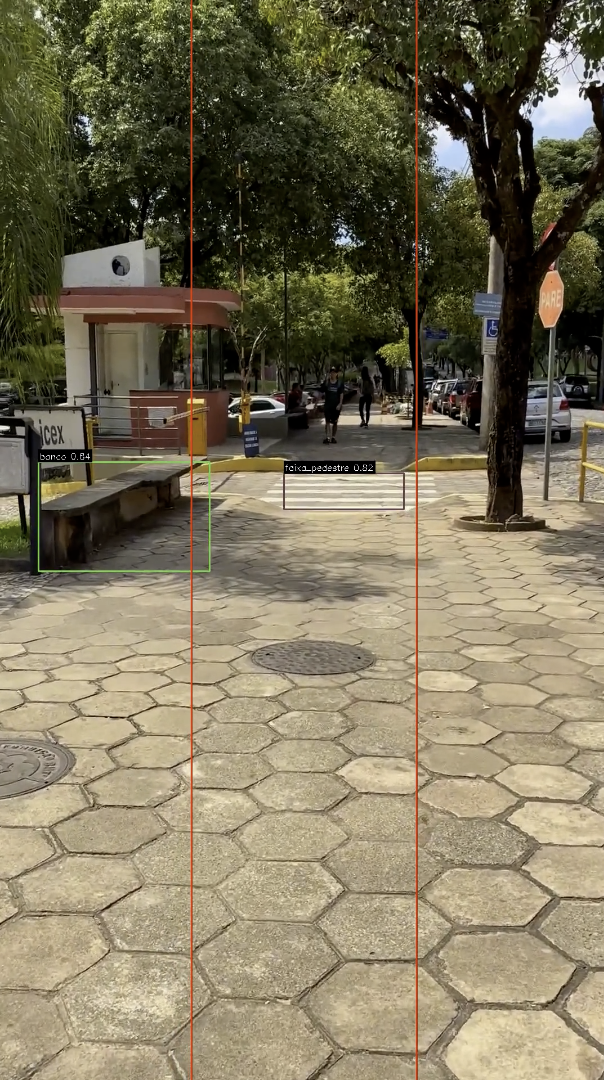
\includegraphics[width=0.6\textwidth]{Figuras/exemplo-deteccao-dia.png}
  \\
  Fonte: Autoral.
  \label{fg-exemplo-deteccao-dia}
\end{figure}
% --- Figura

Em contrapartida, a Figura \ref{fg-baixa_luminosidade} ilustra a atuação do modelo em uma situação de maior complexidade, com baixa iluminação ambiente. Nesse cenário, embora algumas detecções ainda sejam realizadas corretamente — como a identificação de uma placa\_onibus e dois bancos — observou-se uma leve redução na confiança das predições e uma maior variação na \textit{precision} espacial das caixas. Esse comportamento é esperado, dado que condições adversas de iluminação, especialmente à noite, impõem desafios à visão computacional, reduzindo o contraste e a nitidez dos objetos. Apesar disso, o modelo demonstrou capacidade de operar de forma aceitável mesmo sob essas limitações, o que reforça sua aplicabilidade em ambientes reais.

% --- Figura
\begin{figure}[htbp]
  \centering
  \caption{Desempenho do modelo em detecção de objetos sob condições de baixa luminosidade.}
  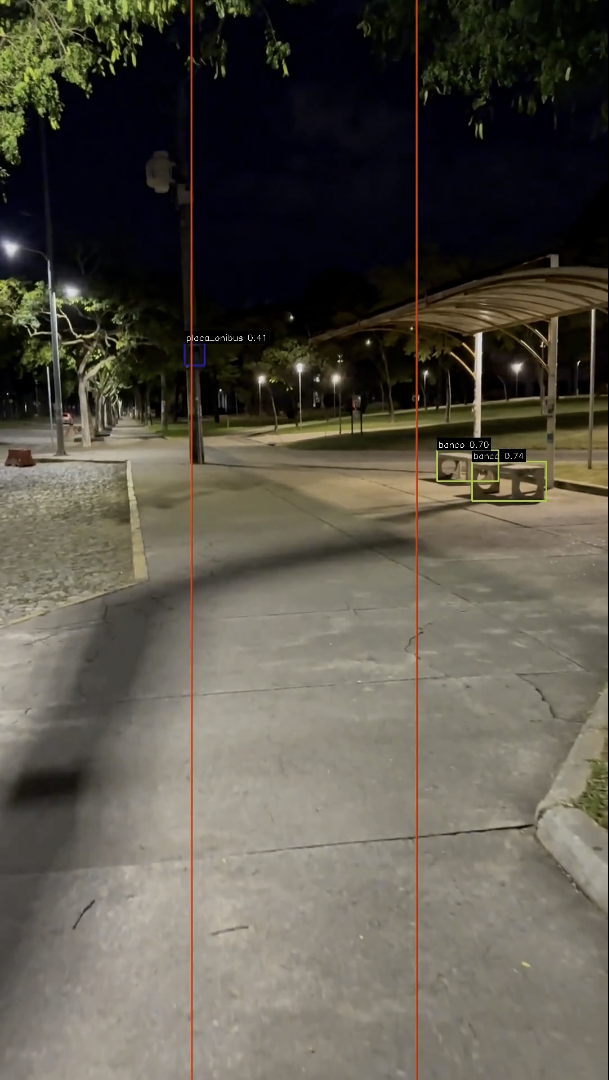
\includegraphics[width=0.6\textwidth]{Figuras/baixa_luminosidade.png}
  \\
  Fonte: Autoral.
  \label{fg-baixa_luminosidade}
\end{figure}
% --- Figura

A Figura 4.9 destaca um caso de falso positivo relacionado à classe faixa de pedestre. A imagem mostra uma região com elementos visuais semelhantes à aparência de uma faixa de pedestre (como listras brancas em cima de cada degrau), que foram incorretamente detectados como tal. Este tipo de equívoco pode ser reduzido no futuro com a inclusão de exemplos negativos mais específicos durante o treinamento ou pela aplicação de ajustes no limiar de confiança da inferência para essa classe.

% --- Figura
\begin{figure}[htbp]
  \centering
  \caption{Exemplo de um Falso Positivo para a classe 'faixa\_pedestre', onde o modelo detectou um objeto incorretamente.}
  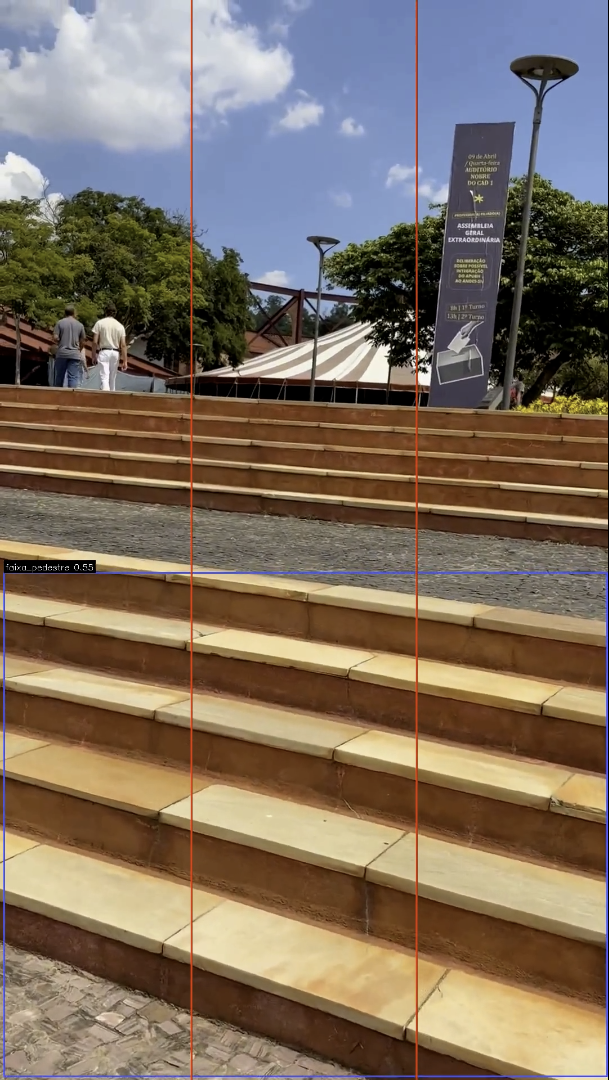
\includegraphics[width=0.6\textwidth]{Figuras/falso_positivo.png}
  \\
  Fonte: Autoral.
  \label{fg-falso_positivo}
\end{figure}
% --- Figura

Na Figura \ref{fg-falso_negativo}, evidencia-se um caso de falso negativo, em que uma faixa\_pedestre claramente visível não foi detectada pelo modelo. A provável causa está associada à condição de baixa iluminação e à presença de sombras que encobrem parcialmente o objeto. Tais situações ressaltam a importância da diversidade do \textit{dataset} e da inclusão de exemplos mais desafiadores, especialmente para objetos que sofrem alterações visuais relevantes em função do tempo ou das condições ambientais.

% --- Figura
\begin{figure}[htbp]
  \centering
  \caption{Exemplo de um Falso Negativo, onde o modelo não detectou um objeto presente.}
  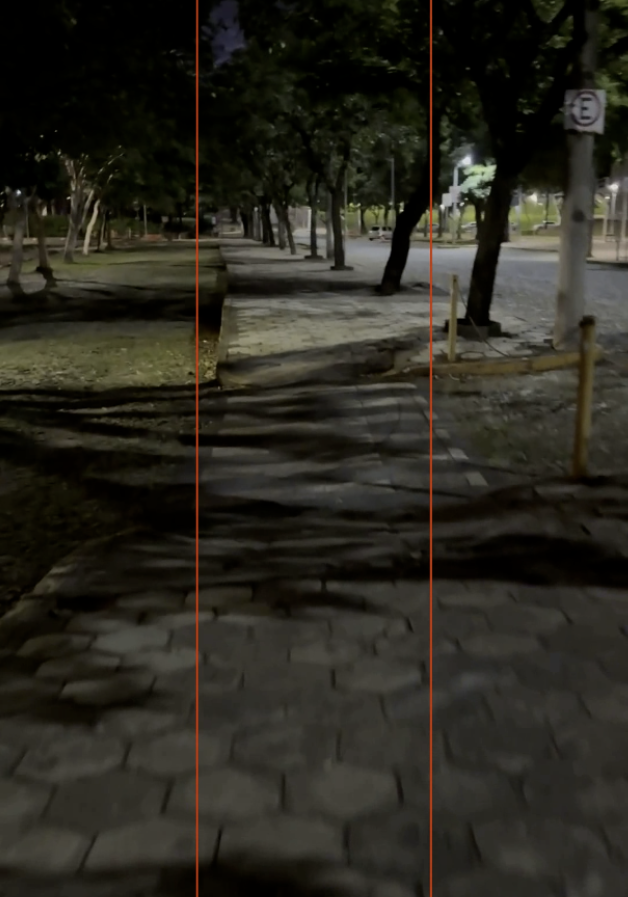
\includegraphics[width=0.6\textwidth]{Figuras/falso_negativo.png}
  \\
  Fonte: Autoral.
  \label{fg-falso_negativo}
\end{figure}
% --- Figura

Conclui-se, com base nesta análise qualitativa, que o modelo é robusto para a maioria dos cenários de uso previstos, mas que ainda existem oportunidades de melhoria, especialmente na redução de falsos positivos da classe banco e faixa de pedestre e no aumento da sensibilidade do modelo em situações de iluminação comprometida. Essas observações visuais corroboram os achados estatísticos apresentados nos tópicos anteriores e oferecem subsídios práticos para ajustes na implementação final do sistema assistivo.

\section{\textbf{Discussão Consolidada dos Resultados e Implicações para a Ferramenta Assistiva}}

A consolidação das análises quantitativa e qualitativa permite uma avaliação abrangente do modelo no que diz respeito à sua viabilidade como núcleo de uma ferramenta assistiva para pessoas com deficiência visual no campus da UFMG. Os resultados obtidos ao longo das avaliações apontam para um desempenho consistente, com alto potencial de aplicação prática e algumas limitações pontuais que podem ser endereçadas em fases posteriores do projeto.

O treinamento do modelo mostrou-se eficaz, com as curvas de perda e de mAP indicando um processo de aprendizagem estável, sem indícios de \textit{overfitting}. As métricas consolidadas no conjunto de validação, como o mAP@0.5 de 0.944 e o mAP@0.5:0.95 de 0.672, colocam o modelo em um patamar competitivo para aplicações reais, especialmente considerando que foi treinado com um volume relativamente modesto de dados. O uso da arquitetura YOLOv11, aliada a um \textit{dataset} bem curado e técnicas de \textit{data augmentation}, demonstrou ser uma escolha acertada, capaz de equilibrar velocidade de inferência e precisão.

No plano das métricas individuais, o desempenho foi particularmente elevado para a classe placa\_onibus, com valores próximos à perfeição em \textit{precision} e \textit{recall}. As classes faixa\_pedestre e banco também apresentaram bons resultados, ainda que a última tenha exibido maior propensão a falsos positivos. Isso indica que, embora o modelo tenha aprendido bem a distinguir visualmente as classes, algumas ambiguidades visuais ainda geram confusões com o fundo. Esse ponto poderá ser refinado com novos ciclos de treinamento, ajustes no limiar de confiança ou por meio de técnicas mais avançadas de regularização.

A análise das curvas de \textit{precision}-\textit{recall} e de \textit{F1-Score} reforçou a qualidade do modelo e ainda ofereceu um subsídio valioso para calibragem prática do sistema: a escolha de um limiar de confiança em torno de 0.4-0.5 tende a maximizar o equilíbrio entre acertos e erros. Essa configuração é especialmente relevante em aplicações assistivas, onde o excesso de alertas incorretos pode gerar desconfiança, e a omissão de objetos críticos pode comprometer a segurança do usuário. Assim, essa análise estatística apoia diretamente as decisões de projeto na integração da detecção com o sistema de \textit{background} auditivo.

As observações visuais das detecções, por sua vez, confirmam que o modelo é funcional em diversos cenários do campus, inclusive em horários noturnos e em ambientes parcialmente oclusos. Ainda que haja margem para melhorias, os resultados indicam que a ferramenta assistiva baseada nesse modelo tem potencial real para contribuir com a autonomia e a mobilidade de pessoas com deficiência visual. A velocidade de inferência, próxima de 20 a 30ms por imagem em ambiente de GPU, sugere viabilidade inclusive para aplicações futuras em tempo real, desde que se utilize \textit{hardware} com capacidade compatível.

Em síntese, o modelo desenvolvido atende de forma satisfatória aos objetivos propostos neste trabalho. Suas limitações são específicas, bem compreendidas e tecnicamente solucionáveis. A base técnica construída ao longo do projeto estabelece um ponto de partida sólido para a evolução da ferramenta, seja por meio de refinamento contínuo do modelo, integração com sensores complementares ou validação com usuários reais em ambientes de uso.